
L'estimation des paramètres de régularité locale en $t_2$ ( $H_{t_2}$ et $L_{t_2}$ ) utilise les incréments quadratiques $\theta$ entre les différents points $t_1, t_2, t_3$ situés dans un voisinage de diamètre $\Delta$ autour de $t_2$.
En observant que $L$ est estimée par une expression impliquant $\theta$ et $\Delta^{2 H}$, une estimation précise de $H$ paraît plus cruciale pour la bonne estimation conjointe des deux quantités. 

\question{
	\smallskip\centering
	Doit-t-on se concentrer sur l'estimation de $H$ ou de $\theta$ ?
}

Les incréments quadratiques $\theta$ sont utilisées à la fois pour l'estimation de $H$ et de $L$. Nous allons donc chercher à déterminer un $\Delta$ adapté à l'estimation des incréments quadratiques. En effet, un mauvaise estimation des incréments induirait une mauvaise estimation de $H$. Puisque l'on a déterminé qu'une bonne estimation de $H$ était cruciale, et que cette quantité utilise deux valeurs d'incréments distinctes, nous allons nous focaliser sur l'estimation d'un couple de $\theta$ que nous noterons $\Theta$.

\bigskip

Le but étant d'obtenir un $\Delta$ utile en pratique, nous réalisons une simulation de Monte-Carlo avec $mc=200$ réplications indépendantes de la procédure d'estimation des paramètres de régularité locale. Et nous cherchons alors à déterminer quel $\Delta$ est meilleur en pratique sur les données simulées.

\bigskip

La métrique que nous allons sélectionner est \emph{la distance euclidienne entre une estimation d'un tel couple $\Theta$, que l'on nomme $\widehat \Theta$ et l'estimateur de l'espérance via la moyenne empirique des courbes non bruitées, observées pleinement, \textbf{relativement} à la cible de l'estimation $\widetilde \Theta$}. En effet, il s'agit du meilleur estimateur de l'espérance que l'on pourrait espérer atteindre (du biais est introduit lors du lissage non paramétrique des courbes bruitées). On considère donc le risque suivant :


\begin{equation}
	{\mathds E_p} \frac{{\distnorme 2 {\widehat \Theta\bigl[\, p \,\bigr]} {\widetilde \Theta \bigl[ \,p \,\bigr]}}^2}{{\norme 2 {\widetilde \Theta \bigl[ \,p \,\bigr]}}^2}
	=
	{\mathcal R} \bigl( \, \Theta \, , \, \Delta \, \bigr)
	\simeq
	\widehat{\mathcal R} \bigl( \, \Theta \, , \, \Delta \, \bigr)
	=
	\frac 1 {mc} \sum\limits_{p=1}^{mc} \frac{{\distnorme 2 {\widehat \Theta\bigl[\, p \,\bigr]} {\widetilde \Theta \bigl[ \,p \,\bigr]}}^2}{{\norme 2 {\widetilde \Theta \bigl[ \,p \,\bigr]}}^2}
\end{equation}

\begin{figure}[H]
	\centering
	\begin{minipage}{0.65\textwidth}
		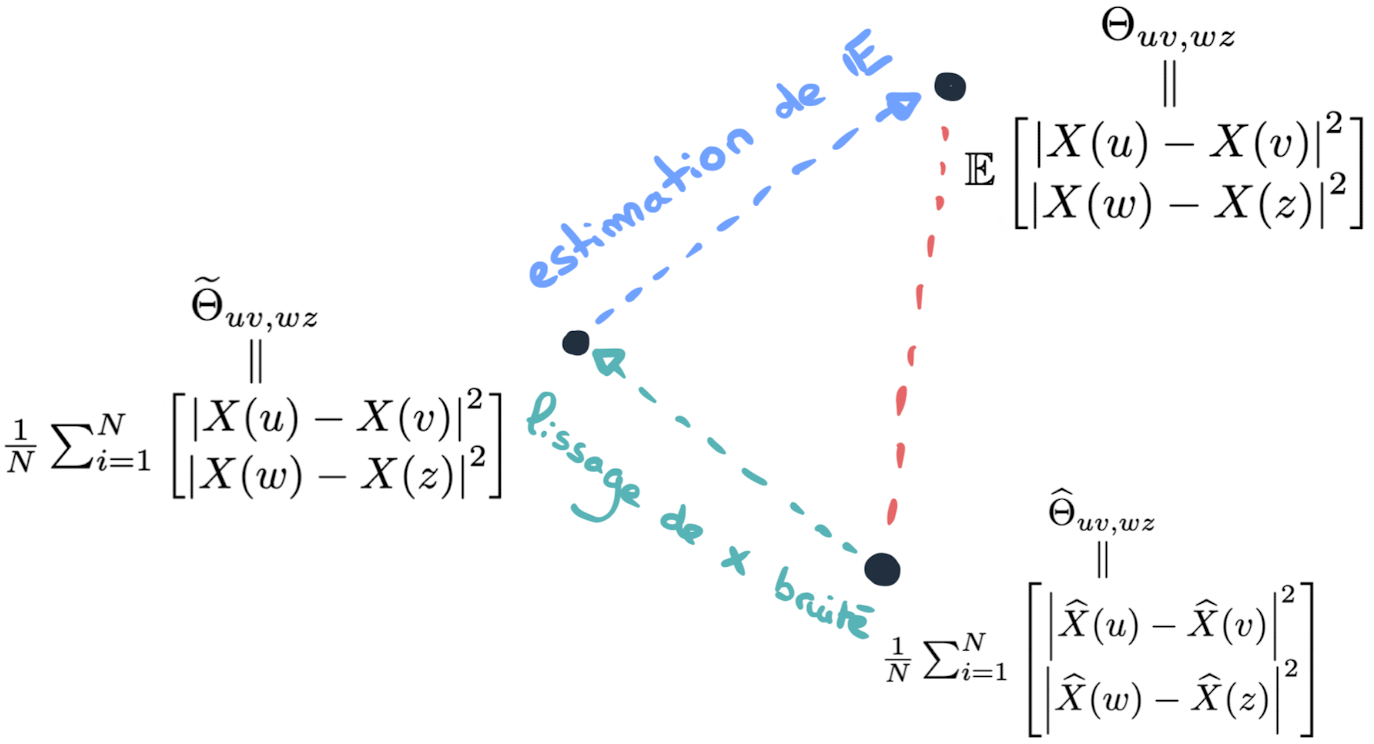
\includegraphics[width=0.8\textwidth]{Images/sketches/theta_biais.png}
	\end{minipage}
	\begin{minipage}{0.3\textwidth}
		Dans la formulation du risque, 
		$[p]$ désigne la $p^{eme}$ réplication de Monte-Carlo de la quantité considérée.
	\end{minipage}
	\caption{Schéma représentant les différentes approximations du couple d'incréments}
	\label{fig:sketch_theta_biais_corpus}
\end{figure}
